\documentclass[tikz,border=8pt]{standalone}
\usepackage{xcolor}
\usetikzlibrary{calc,arrows.meta,backgrounds}
\definecolor{bg}{HTML}{1B1F27}
\definecolor{fg}{HTML}{E6EDF3}
\definecolor{dim}{HTML}{9AA5B1}
\definecolor{c1}{HTML}{7BC47F}
\definecolor{c2}{HTML}{E5826F}
\definecolor{feat}{HTML}{F0C060}
\begin{document}
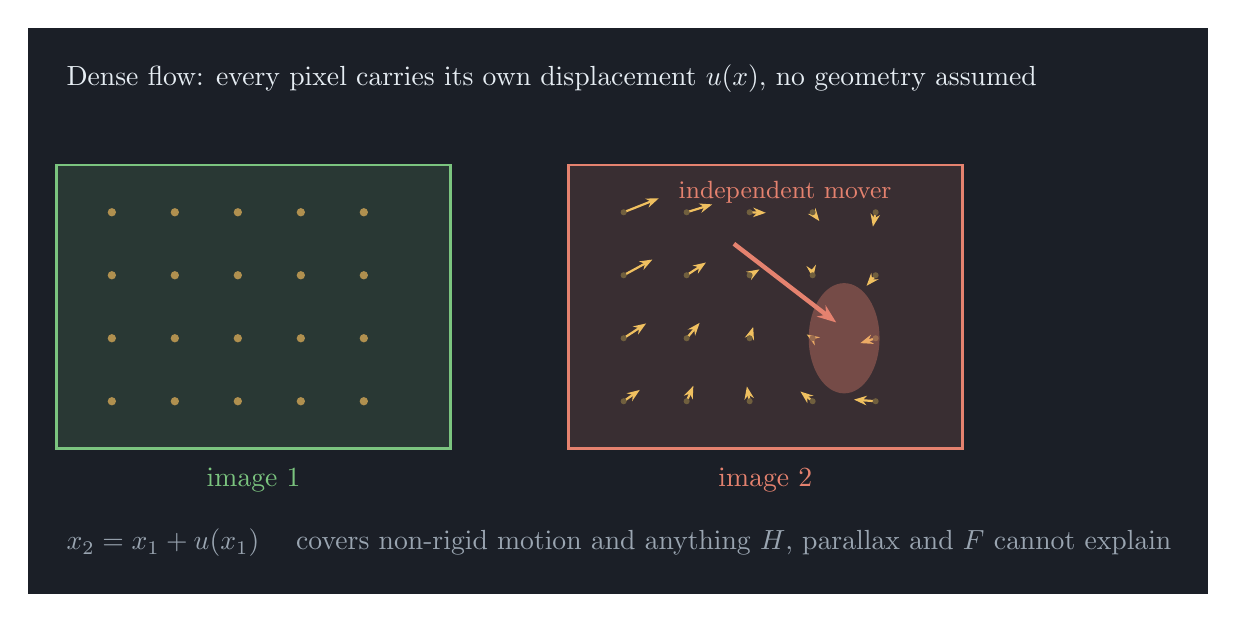
\begin{tikzpicture}[show background rectangle, background rectangle/.style={fill=bg}, inner frame sep=10pt, every node/.style={text=fg}]
\draw[c1, line width=1pt, fill=c1!15!bg] (0,0) rectangle (5,3.6);
\draw[c2, line width=1pt, fill=c2!15!bg] (6.5,0) rectangle (11.5,3.6);
\node[text=c1] at (2.5,-0.4) {image 1};
\node[text=c2] at (9,-0.4) {image 2};
\foreach \x in {0.7,1.5,2.3,3.1,3.9}{
  \foreach \y in {0.6,1.4,2.2,3.0}{
    \fill[feat!70!bg] (\x,\y) circle (1.5pt);
    \pgfmathsetmacro{\dx}{0.25+0.1*\y-0.15*\x}
    \pgfmathsetmacro{\dy}{0.2*sin(40*\x+30*\y)}
    \draw[-{Stealth[length=1.6mm]}, feat, line width=0.8pt] (6.5+\x,\y) -- ++(\dx,\dy);
    \fill[feat!40!bg] (6.5+\x,\y) circle (1.1pt);
  }
}
\fill[c2, opacity=0.35] (10.0,1.4) ellipse (0.45 and 0.7);
\draw[-{Stealth[length=2.4mm]}, line width=1.6pt, c2] (8.6,2.6) -- (9.9,1.6);
\node[text=c2, font=\small] at (9.25,3.25) {independent mover};
\node[anchor=west] at (0,4.7) {Dense flow: every pixel carries its own displacement $u(x)$, no geometry assumed};
\node[anchor=west, text=dim] at (0,-1.2) {$x_2=x_1+u(x_1)$ \quad covers non-rigid motion and anything $H$, parallax and $F$ cannot explain};
\end{tikzpicture}
\end{document}
